%\title{LaTeX Portrait Poster Template}
%%%%%%%%%%%%%%%%%%%%%%%%%%%%%%%%%%%%%%%%%
% a0poster Portrait Poster
% LaTeX Template
% Version 1.0 (22/06/13)
%
% The a0poster class was created by:
% Gerlinde Kettl and Matthias Weiser (tex@kettl.de)
% 
% Adapter by Jens Buysse for Hogeschool Gent
% This template has been downloaded from:
% http://www.LaTeXTemplates.com
%
% License:
% CC BY-NC-SA 3.0 (http://creativecommons.org/licenses/by-nc-sa/3.0/)
%
%%%%%%%%%%%%%%%%%%%%%%%%%%%%%%%%%%%%%%%%%

%----------------------------------------------------------------------------------------
%	PACKAGES AND OTHER DOCUMENT CONFIGURATIONS
%----------------------------------------------------------------------------------------

\documentclass[a0,portrait]{a0poster}

\usepackage{multicol} % This is so we can have multiple columns of text side-by-side
\columnsep=100pt % This is the amount of white space between the columns in the poster
\columnseprule=3pt % This is the thickness of the black line between the columns in the poster

\usepackage[svgnames]{xcolor} % Specify colors by their 'svgnames', for a full list of all colors available see here: http://www.latextemplates.com/svgnames-colors

\usepackage{times} % Use the times font
%\usepackage{palatino} % Uncomment to use the Palatino font

\usepackage{graphicx} % Required for including images
\graphicspath{{figures/}} % Location of the graphics files
\usepackage{booktabs} % Top and bottom rules for table
\usepackage[font=small,labelfont=bf]{caption} % Required for specifying captions to tables and figures
\usepackage{amsfonts, amsmath, amsthm, amssymb} % For math fonts, symbols and environments
\usepackage{wrapfig} % Allows wrapping text around tables and figures
\usepackage[export]{adjustbox}
\usepackage[none]{hyphenat}
\begin{document}

%----------------------------------------------------------------------------------------
%	POSTER HEADER 
%----------------------------------------------------------------------------------------

% The header is divided into two boxes:
% The first is 75% wide and houses the title, subtitle, names, university/organization and contact information
% The second is 25% wide and houses a logo for your university/organization or a photo of you
% The widths of these boxes can be easily edited to accommodate your content as you see fit

\begin{minipage}[t]{0.75\linewidth}
\VeryHuge \color{HoGentAccent1} \textbf{Automatische transformatie van ingescande tabellen naar gestructureerde digitale data} \color{Black}\\ % Title
\Huge\textit{Een proof-of-concept}\\[2.4cm] % Subtitle
\huge \textbf{Nazari Milad, Bram Vandewalle, Martijn Saelens}\\[0.5cm] % Author(s)
\huge Hogeschool Gent, Valentin Vaerwyckweg 1, 9000 Gent\\[0.4cm] % University/organization
\Large \texttt{contact@miladnazari.be} \\
\end{minipage}
%
\begin{minipage}[t]{0.25\linewidth}
\includegraphics[width=13cm,right]{figures/HOGENT_Logo_Pos_rgb.png} 

\end{minipage}

\vspace{1cm} % A bit of extra whitespace between the header and poster content

%----------------------------------------------------------------------------------------

\begin{multicols}{2} % This is how many columns your poster will be broken into, a portrait poster is generally split into 2 columns

%----------------------------------------------------------------------------------------
%	ABSTRACT
%----------------------------------------------------------------------------------------

\color{HoGentAccent1} % Navy color for the abstract

\begin{abstract}
\noindent Met dit onderzoek wordt het ontwerp en ontwikkeling van een open source prototype-software bestudeerd die het mogelijk zou maken om tabellen in ingescande documenten te digitaliseren. Dit zou niet enkel digitaliseringsprocessen versnellen maar zou het eveneens gebruikt kunnen worden voor verschillende digitalisatietaken, zoals de digitalisatie van medicatieschema’s. Er wordt eerst een literatuurstudie uitgevoerd om de stand van zaken rond tabeltransformatie te verduidelijken. Vervolgens worden systeemvereisten en non-goals voor de proof-of-concept gespecifieerd. Op basis hiervan worden de algoritmes voor tabeltransformatie en de technologieën geselectioneerd. Hierna wordt de proof-of-concept in detail toegelicht, bovendien werd een nieuwe algoritme voorgesteld voor structuuranalyse. Uiteindelijk wordt de software op een dertig tal afbeeldingen getest. Hoewel bij de test alle tabellen juist gedetecteerd worden, wordt de nauwkeurigheid van de tabeltransformatie verlaagd door de minder performante tabelstructuuranalyse. De voorgestelde nieuwe algoritme echter verhoogt de nauwkeurigheid van de structuuranalyse, al kan hierdoor de software nog niet als perfect beschouwd worden. Men kan bij dit onderzoek concluderen dat tabeltransformatie een complex domein is. Kant en klaar software-pakketten bestaan, maar zijn betalend en niet open source. Verder kan besloten worden dat tabelstructuuranalyse uit meerdere, van elkaar afhankelijke, subprocessen bestaat. Tenslotte kan men concluderen dat tabeldetectie enerzijds zeer nauwkeurig is, terwijl anderzijds structuuranalyse minder optimale resultaten kan leveren. De voorgestelde algoritme die een niet onbelangrijke verbetering van de tabeltransformaties teweegbrengt, toont aan dat optimalisatiemogelijkheden zeker nog mogelijk zijn.
\end{abstract}
%----------------------------------------------------------------------------------------
%	INTRODUCTION
%----------------------------------------------------------------------------------------

\color{HoGentAccent1} 
\section*{Introductie}
\color{black}
\color{black}
Alhoewel meer en meer processen wereldwijd volledig digitaal plaatsvinden, worden toch nog een grote deel van procedures en data opslag uitgevoerd op niet-digitale manieren. Zo krijgen de meeste mensen en bedrijven hun factures nog steeds per brief. Daarbovenop worden kassatickets nog steeds afgedrukt op papier, en notities nemen op papier blijft de populaire keuze hoewel er tal van notitie-apps bestaan. Deze voorbeelden tonen aan dat essentiële data nog massaal op een niet-digitale, en dus niet-automatisch verwerkbare media bewaard wordt, namelijk op papier.\\

\noindent Tot enkele jaren geleden was dit probleem niet zo beduidend maar nu meer digitale platformen voor dataverwerking gebruikt worden, is het omzetten van data op papier naar digitale data, m.a.w. het digitalisatieproces steeds belangrijker geworden. Tot heden bestaat er geen open source oplossing die tabellen in foto’s transformeert naar digitale tabellen, m.a.w. naar digitale structuren waarbij de tekst, evenals de relatie tussen de verschillende teksten getransformeerd wordt. Daarom werd er voor deze bachelorproef besloten om een proof-of-concept van een tabeltransformatiesoftware te creëren die bij een foto automatisch tabellen detecteert en deze tabellen digitaliseert.\\ \\

\begin{center}\vspace{1cm}
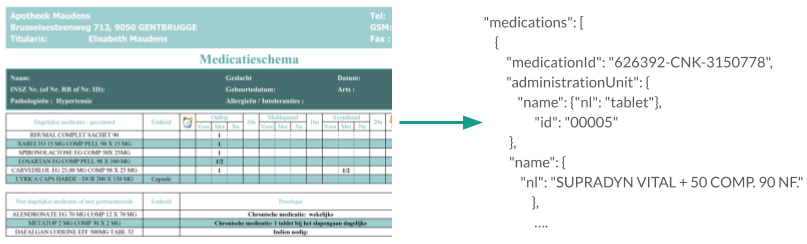
\includegraphics[width=1.0\linewidth]{tabel_transformatie.png}
\captionof{figure}{\color{HoGentAccent5} Tabeltransformatie}
\end{center}\vspace{1cm}

\noindent Een open source tabeltransformatiesoftware zal automatisch bijv. medicatieschema’s kunnen omzetten in een uniform digitale datastructuur, zoals weergegeven in bovenstaande figuur. Hierdoor zal er geen manuele werk uitgevoerd moeten worden, wat tijd- en kostenreductie als positieve gevolgd heeft. Daarbovenop, omdat het open source zal zijn, zal men niet te maken hebben met softwarelicentiekosten of privacyschendingrisico's. Hoewel het digitaliseren van medicatieschema’s een belangrijke toepassing is, zijn er tal van andere potentiële toepassingen, aangezien tabellen zo vaak gebruikt worden. Zo zou men tabeltransformatie eveneens kunnen gebruiken voor het inscannen van kassatickets, het analyseren van een sudokuspel, het digitaal weergeven van een - op een whiteboard gemarkeerde - matrix voor online leerplatformen, het verwerken van een foto van een voedingswaardetabel op de verpakking van voedsel, en meer.
\color{Black} % DarkSlateGray color for the rest of the content
\color{HoGentAccent1} 
\section*{Proof-of-concept en resultaten}
\color{black}
Zoals de volgende figuur het weergeeft, worden bij de proof-of-concept meerdere processen doorgelopen. Als eerst uploadt de gebruiker een afbeelding naar de transformatieserver d.m.v. de GUI. Vervolgens wordt de afbeelding verwerkt in de preprocessing-stap om de nauwkeurigheid van de tabeltransformatie te verhogen. Hierna worden de tabellen in de afbeelding gedetecteerd m.b.v. een diep neurale netwerk en geïsoleerd. Dan wordt elke geïsoleerd tabel getransformeerd in de structuuranalyse-stap waarin tekstherkenning, lijndetectie, cellsegmentatie en hiërarchische clustering plaatsvinden (voorgestelde algoritme). Een postprocessing-stap wordt eveneens uitgevoerd om de nauwkeurigheid verder te verhogen. Uiteindelijk worden de getransformeerde tabellen in JSON-formaat teruggestuurd naar de gebruiker.

\begin{center}\vspace{1cm}
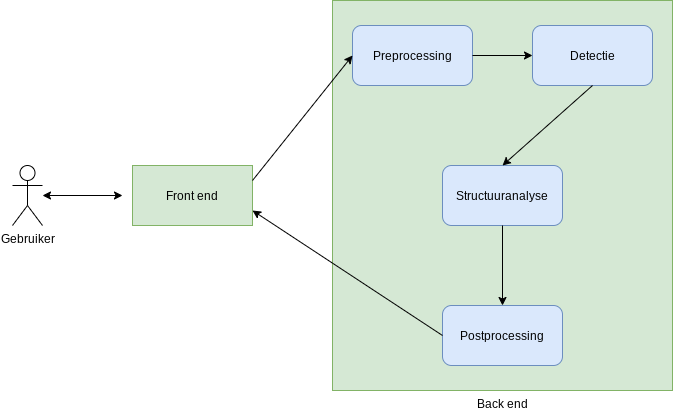
\includegraphics[width=0.8\linewidth]{proof_of_concept_architectuur.png}
\captionof{figure}{\color{HoGentAccent5} Architectuur van de proof-of-concept}
\end{center}\vspace{1cm}

\noindent Hoewel bij de performantietest alle tabellen juist gedetecteerd werden, werd de nauwkeurigheid van de tabeltransformatie verlaagt door de minder performante tabelstructuuranalyse. De voorgestelde algoritme echter verhoogde de nauwkeurigheid van de structuuranalyse, al kan hierdoor de software nog niet als perfect beschouwd worden.

\begin{center}\vspace{1cm}
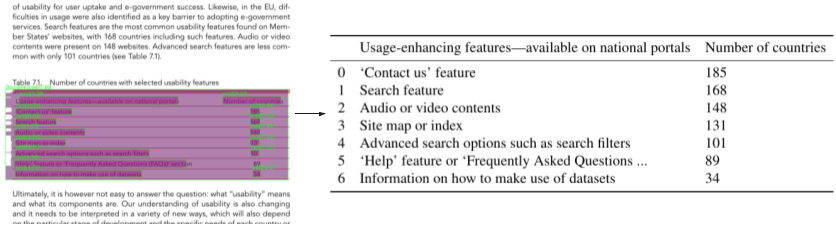
\includegraphics[width=1.0\linewidth]{resultaat_voorbeeld_proof_of_concept.png}
\captionof{figure}{\color{HoGentAccent5} Voorbeeld tabeltransformatie d.m.v. proof-of-concept}
\end{center}\vspace{1cm}

\color{HoGentAccent1} 
\section*{Conclusies}
\color{black}
Men kan bij dit onderzoek concluderen dat tabeltransformatie een complex domein is. Kant en klaar software-pakketten bestaan, maar zijn betalend en niet open source. Een open source versie bestaat momenteel niet. Verder kan besloten worden dat tabelstructuuranalyse niet een simpel eenvoudig proces is. Eerder is het een complex procedure die uit meerdere, van elkaar afhankelijke, subprocessen bestaat. Tenslotte kan men concluderen dat tabeldetectie enerzijds zeer nauwkeurig is, terwijl anderzijds structuuranalyse minder optimale resultaten kan leveren. De voorgestelde algoritme die een niet onbelangrijke verbetering van de tabeltransformaties teweegbrengt, toont aan dat optimalisatiemogelijkheden zeker nog mogelijk zijn.
\color{HoGentAccent1} 
\end{multicols}
\end{document}
